\documentclass[zavrsnirad]{fer}
% LTeX: language=hr-HR
% Dodaj opciju upload za generiranje konačne verzije koja se učitava na FERWeb
% Add the option upload to generate the final version which is uploaded to FERWeb


\usepackage{blindtext}
\usepackage{amssymb}


%--- PODACI O RADU / THESIS INFORMATION ----------------------------------------

% Naslov na engleskom jeziku / Title in English
\title{Demonstrative framework for differenciable programming}

% Naslov na hrvatskom jeziku / Title in Croatian
\naslov{Demonstracijski okvir za diferencijabilno programiranje}

% Broj rada / Thesis number
\brojrada{1665}

% Autor / Author
\author{Jakov Novak}

% Mentor 
\mentor{Prof.\ dr.\ sc.\ Sliniša Šegvić}

% Datum rada na engleskom jeziku / Date in English
\date{June, 2024}

% Datum rada na hrvatskom jeziku / Date in Croatian
\datum{lipanj, 2024.}

%-------------------------------------------------------------------------------


\begin{document}


% Naslovnica se automatski generira / Titlepage is automatically generated
\maketitle


%--- ZADATAK / THESIS ASSIGNMENT -----------------------------------------------

% Zadatak se ubacuje iz vanjske datoteke / Thesis assignment is included from external file
% Upiši ime PDF datoteke preuzete s FERWeb-a / Enter the filename of the PDF downloaded from FERWeb
\zadatak{zadatak.pdf}


%--- ZAHVALE / ACKNOWLEDGMENT --------------------------------------------------

\begin{zahvale}
  % Ovdje upišite zahvale / Write in the acknowledgment
  \textbf{TODO:} napisati zahvalu za obitelj, prijatelje i profesore
\end{zahvale}


% Odovud započinje numeriranje stranica / Page numbering starts from here
\mainmatter


% Sadržaj se automatski generira / Table of contents is automatically generated
\tableofcontents


%--- UVOD / INTRODUCTION -------------------------------------------------------
\chapter{Uvod}
\label{pog:uvod}

\section{Motivacija}
Većina klasičnih postupaka u dubokom učenju se svode na optimizaciju izlaza neuralne mreže s obzirom na neku funkciju gubitka. Kod takvih postupaka je ključan izračun gradijenta te funkcije kako bi se podesile značajke mreže:
\begin{equation}
  \nabla (f \circ L) (ulaz)
\end{equation}
Postoje različiti pristupi u korištenju računala za rješavanje tog problema. Neki od glavnih su: simboličko diferenciranje, numeričke metode i automatska diferencijacija. Glavni nedostatci prvih spomenutih pristupa su prevelika složenost dobivenih izraza (citation needed) i nepreciznost brojeva s pomičnim zarezom (citation needed). Ovaj rad je fokusiran na proučavanju metoda automatske diferencijacije te implementacije jednostavnog demonstracijskog okvira u programskom jeziku C++ uz pomoć biblioteke OpenCL za matrične operacije.

\section{Metode automatske diferencijacije}
Glavna ideja automatske diferencijacije jest da dobivenu matematičku funkciju možemo prikazati kao aciklički digraf kojemu su čvorovi varijable, konstante ili međurezultati: $G = (V, E). V = Var \cup F$, gdje je $Var$ skup varijabli, a $F$ skup primitivnih funkcija koje se lako mogu derivirati. Ulaz neke funkcije $f \in F$ je definiran kao: $\{x \in V \colon (x, f) \in E\}$
\begin{figure}[h]
  \centering
  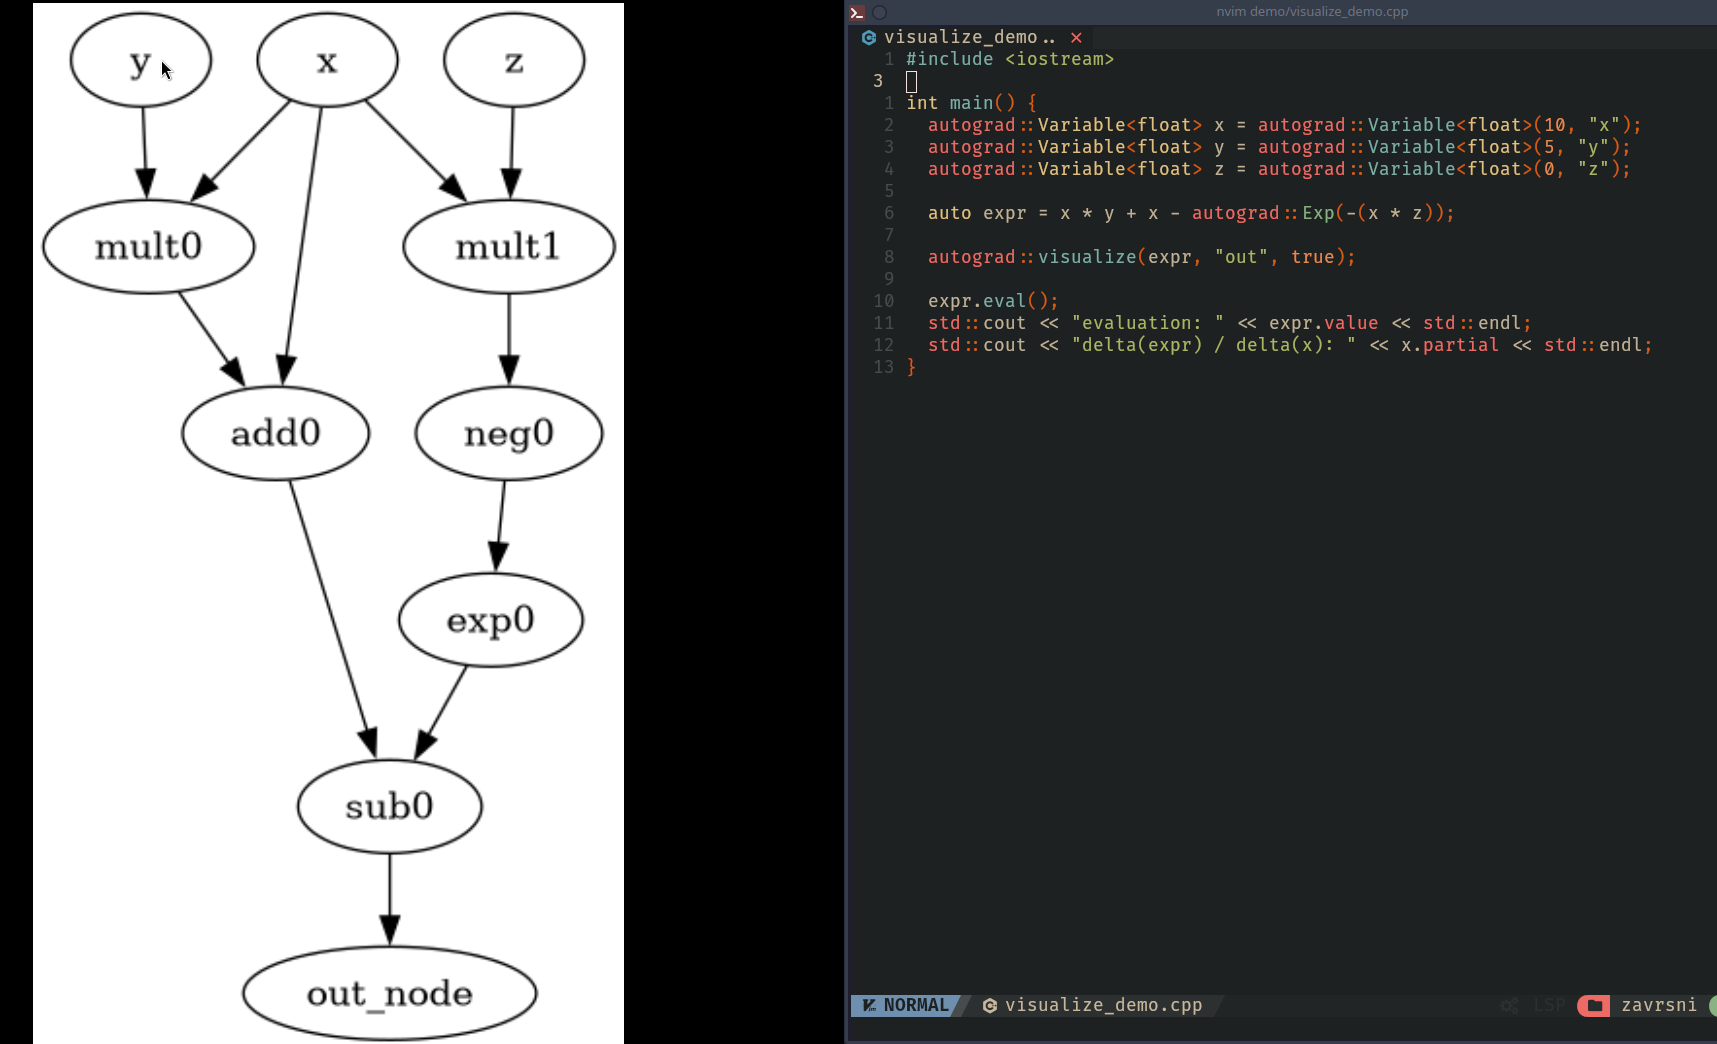
\includegraphics[width=0.7\linewidth]{../../pics/demo1.png}
  \caption{Primjer grafa funkcije: $f(x, y, z) = x * y + x - \exp(-x*z)$}
  \label{slk:graf_funkcije1}
\end{figure}
\\
Općenito, za neku funkciju: $f\colon \mathbb{R}^n \rightarrow \mathbb{R}^m$ vrijedi da će njezin graf imati $n$ čvorova varijabli, odnosno $n$ izvora te $m$ izlaznih čvorova, tj. $m$ ponora. Dodatno možemo pojednostaviti njezin graf ako funkciju zamislimo kao $f\colon \mathbb{V}^n \rightarrow \mathbb{V}^m$ te zatim predstavimo sve varijable kao vektore. Ta ideja će nam uvelike pojednostaviti samu implementaciju autograd programa jer će apstrahirati prijelaz s univarijatnih na multivarijatne funkcije.
\\
Sa slike \ref{slk:graf_funkcije1} možemo već naslutiti koja je glavna ideja algoritma; Glavna ideja jest da obiđemo zadani graf te u svakom čvoru odredimo derivaciju po pravilu ulančavanja:
\begin{equation}
  \frac{\partial (f_1 \circ (f_2 \circ \dotsb (f_{n-1} \circ f_n)))}{\partial x}
    = \frac{\partial f_1}{\partial f_2} \frac{\partial f_2}{\partial f_3}
      \dotsb
      \frac{\partial f_{n-1}}{\partial f_n} \frac{\partial f_n}{\partial x}
\end{equation}
\\
\subsection{Forward mode}
Ovdje postoje dva pristupa: prvi, takozvani \textit{forward mode accumulation}, jest da počnemo od čvorova ulaza prema čvorovima izlaza, po formuli:
\begin{equation}
  \frac{\partial (f_{i-1} \circ f_i)}{\partial x} = \frac{\partial f_{i-1}}{\partial x} \frac{\partial f_i}{\partial f_{i-1}}
\end{equation}
\begin{figure}[h]
  \centering
  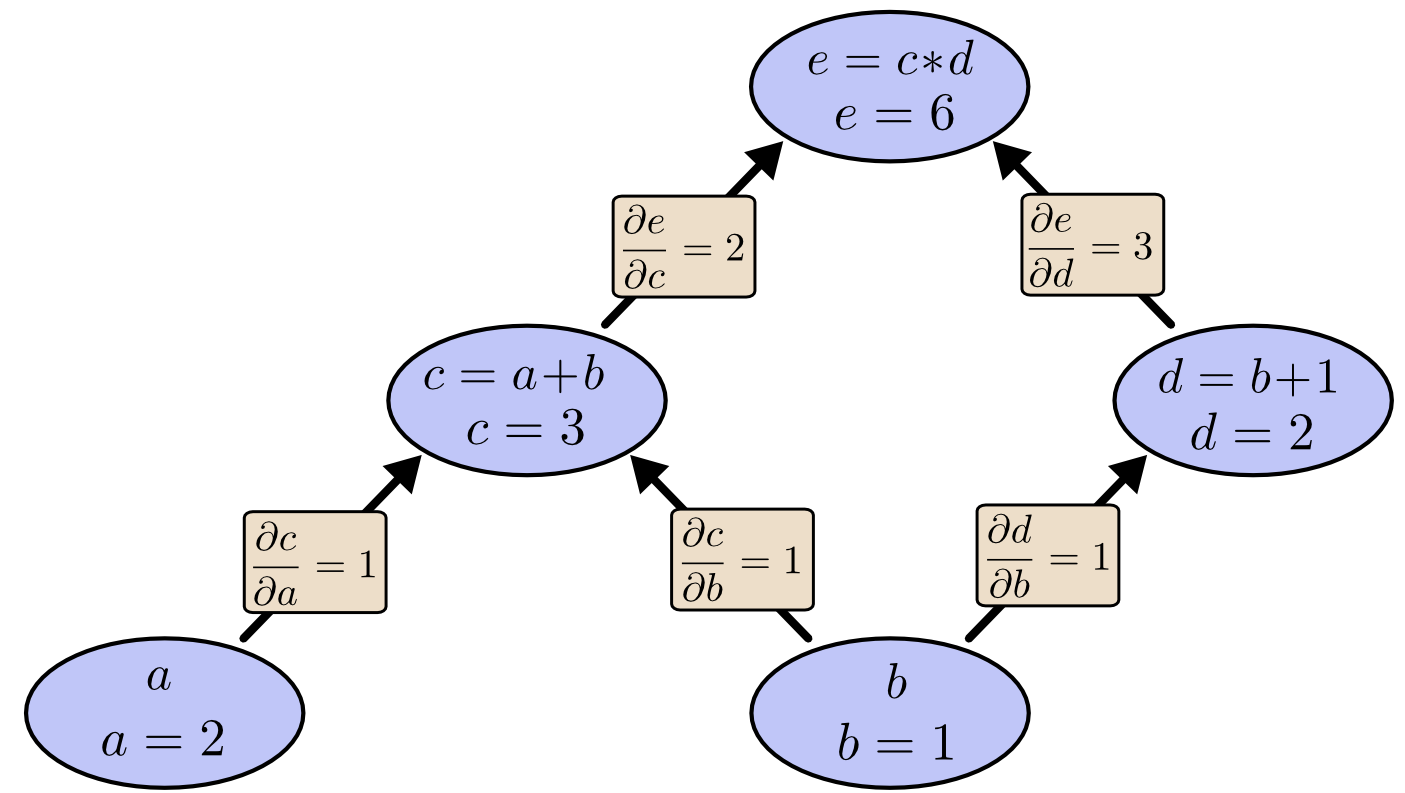
\includegraphics[width=0.7\linewidth]{"./slike/forward_graph.png"}
  \caption{slika preuzeta s: http://wuciawe.github.io/math/2017/02/08/notes-on-differentiation.html}
  \label{slk:forward_graph}
\end{figure}
Vrijednost $f_{i-1}$ je u početku jednaka 1, a kasnije se propagira kroz slojeve grafa \ref{slk:forward_graph} kao vrijednost koju u literaturi često nazivaju \textit{seed value} (citation needed). Ovaj pristup je pogodan ukoliko je broj ulaza daleko manji od broja izlaza, odnosno vrijedi $f\colon \mathbb{R}^n \rightarrow \mathbb{R}^m. n << m$. Složenost ovog koda ovisi o strukturi grafa, no vidljivo je da prolazak kroz graf ponavljamo $n$ puta te je stoga poželjno da je $n$ mnogo manji od $m$. Ovaj pristup nije idealan za strojno učenje pošto je često ulazna domena mnogo veća od izlazne u toj primjeni.
\\
\subsection{Reverse mode}
Drugi pristup problemu automatske diferencijacije jest takozvani \textit{reverse mode accumulation}, tj. prolazak grafa unazad:
\begin{equation}
  \frac{\partial (f_i \circ f_{i+1})}{\partial x} = \frac{\partial f_{i+1}}{\partial f_i} \frac{\partial f_i}{\partial x}
\end{equation}
\begin{figure}[h]
  \centering
  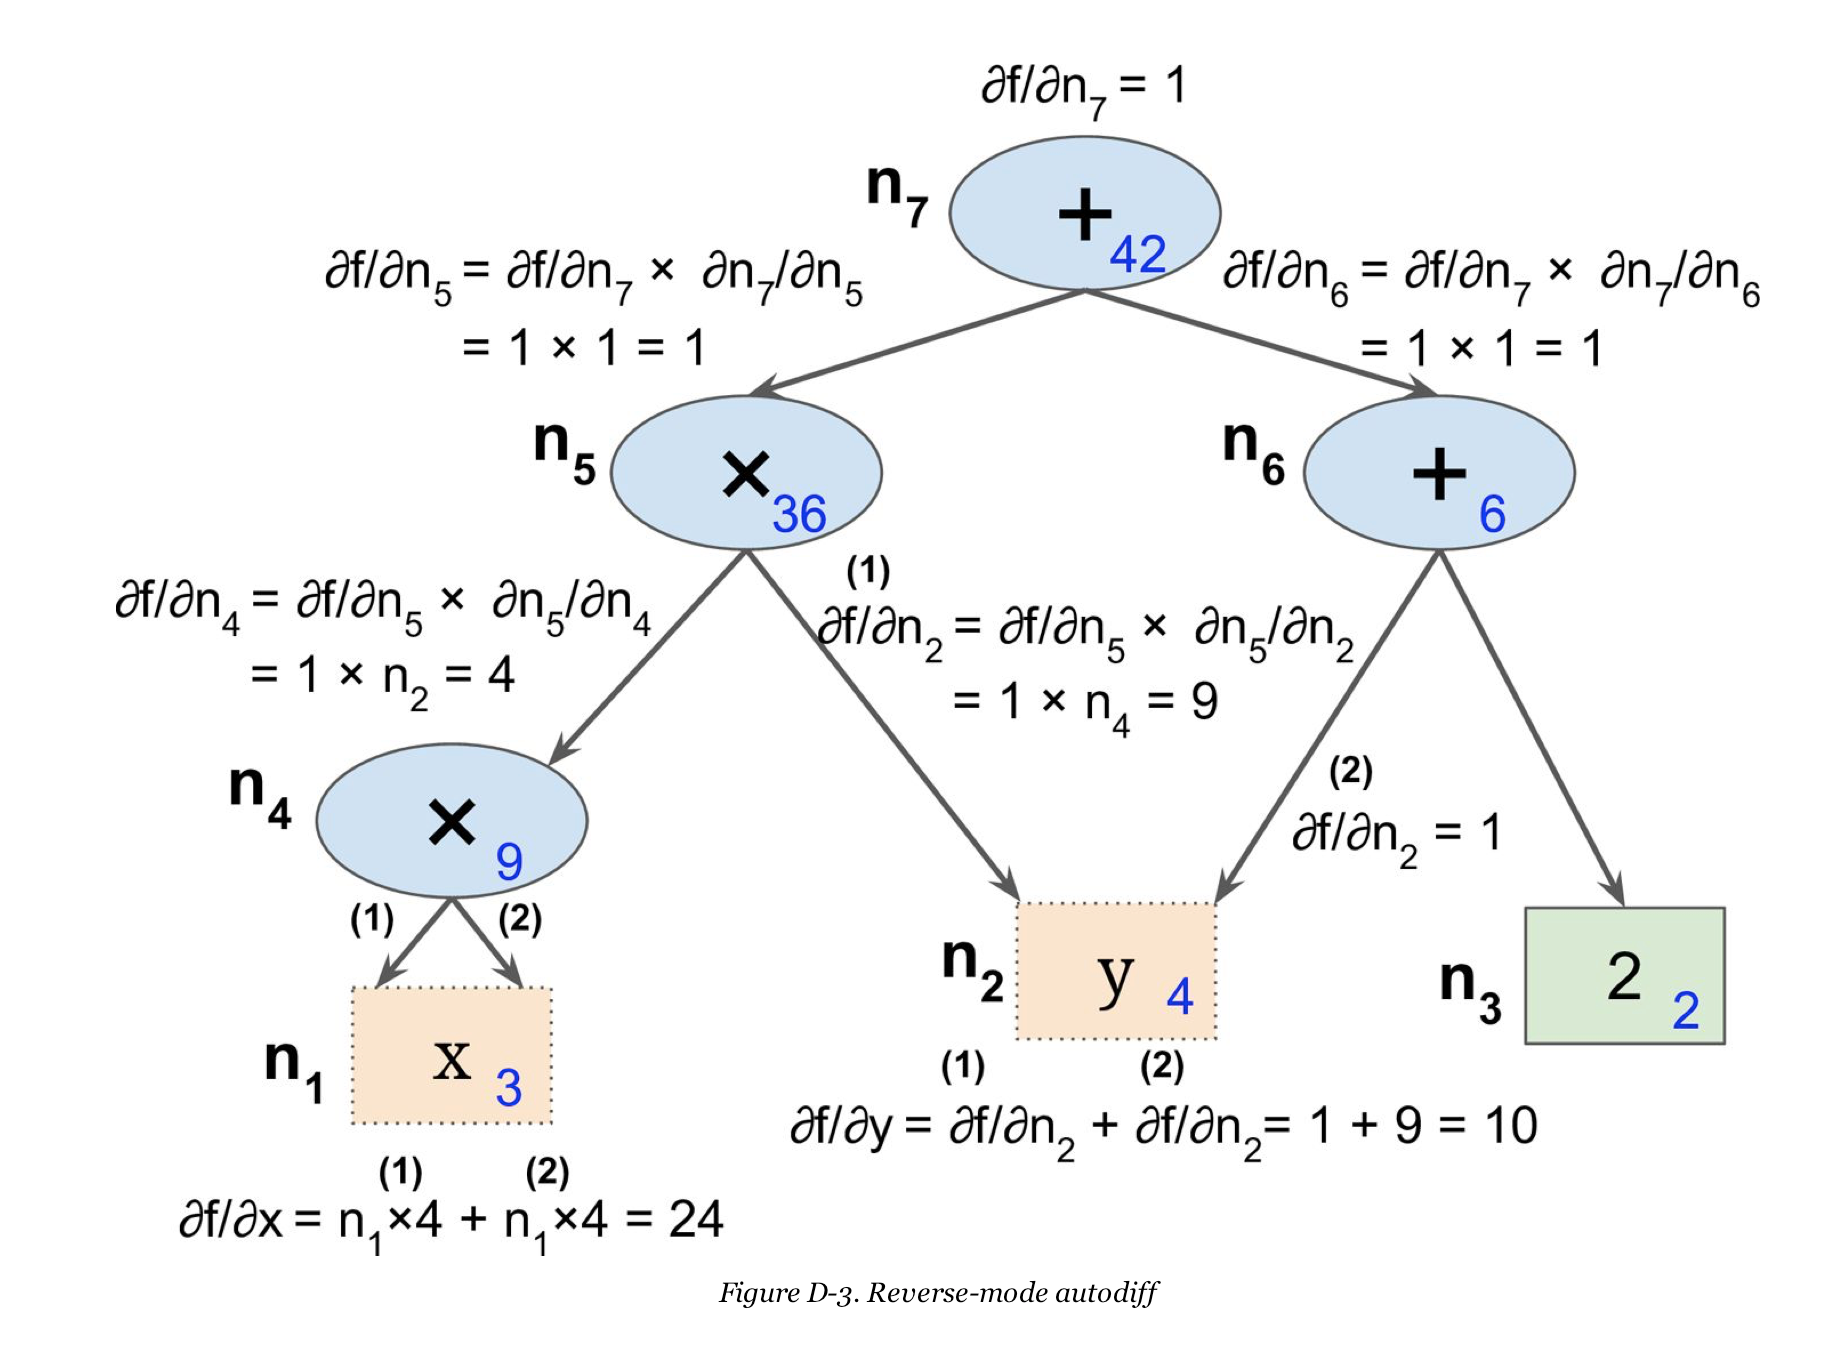
\includegraphics[width=0.7\linewidth]{"./slike/reverse_graph.png"}
  \caption{slika preuzeta s: https://srijithr.gitlab.io/post/autodiff/}
  \label{slk:reverse_graf}
\end{figure}
U ovom pristupu se \textit{seed}-vrijednost šalje unazad kroz graf jednadžbe od ponora prema izvorima \ref{slk:reverse_graf}. Iz toga slijedi da će za neku funkciju $f\colon \mathbb{R}^n \rightarrow \mathbb{R}^m. m << n$ algoritam biti najefikasniji zato što će se $m$ puta pozvati funkcija prolaska kroz graf. Poseban slučaj ovog pristupa problemu automatske diferencijacije jest temeljni princip koji se koristi za unazadnu propagaciju (\textit{eng. backpropagation}) u strojnom učenju (\textbf{citation needed}).
\\
Zanimljivo je da su oba algoritma optimalna samo za jednu određenu domenu primjene. To je zato što je problem izračuna Jakobijana za proizvoljnu funkciju $f\colon \mathbb{R}^n \rightarrow \mathbb{R}^m$ s minimalnim brojem računskih operacija problem koji je NP-potpun. Problem je poznat i kao \textit{optimal Jacobian problem}.
\textbf{citation needed za ovo zadnje}
\textbf{pseudokod za oba pristupa?}

\section{Dualni brojevi}
\textbf{TODO:} napiši nekaj o dualnim brojevima
\textbf{pseudokod za ovaj pristup?}
\\
\blindtext

\section{Pristupi implementaciji grafa}
\textbf{TODO:} opiši IR vs Operator overloading...
\\
\blindtext

\section{OpenCL i C++}
\textbf{TODO:} napiši nekaj tu...
\\
\blindtext


%-------------------------------------------------------------------------------
\chapter{Glavni dio}
\label{pog:glavni_dio}

\section{Autograd\_core implementacija}
\textbf{TODO:} opiši jezgrenu funkcionalnost i zakaj je taksa
\blindtext

\section{Matrix calculus}
\textbf{TODO:} opiši matrične operacije i poveži ih s matematičkom analizom
\blindtext

\section{OpenCL + autograd\_core}
\textbf{TODO:} opiši kak si povezal opencl i autograd core implementaciju
\blindtext

\section{Demonstracijski programi}
\textbf{TODO:} izdvoji najbitnije demonstracijske programe koje si napisal
\blindtext

%-------------------------------------------------------------------------------
\chapter{Rezultati i rasprava}
\label{pog:rezultati_i_rasprava}

\section{Usporedba s pytorchem}
\textbf{TODO:} usporedi brzinu izvođenja demonstracijskih programa s pytorch ekvivalentima
\blindtext

\section{Moguće optimizacije}
\textbf{TODO:} piši o mogućim optimizacijama pretraživanja grafa. recimo odsjecanje grana itd.
\blindtext

\section{Budući rad}
\textbf{TODO:} opiši kaj si mogel još dodati u smislu featurea
cite test
\blindtext


%--- ZAKLJUČAK / CONCLUSION ----------------------------------------------------
\chapter{Zaključak}
\label{pog:zakljucak}

Zaključno, TODO...
\blindtext


%--- LITERATURA / REFERENCES ---------------------------------------------------

% Literatura se automatski generira iz zadane .bib datoteke / References are automatically generated from the supplied .bib file
% Upiši ime BibTeX datoteke bez .bib nastavka / Enter the name of the BibTeX file without .bib extension
\bibliography{literatura}



%--- SAŽETAK / ABSTRACT --------------------------------------------------------

% Sažetak na hrvatskom
\begin{sazetak}
  \textbf{TODO:} Unesite sažetak na hrvatskom.
  \blindtext
\end{sazetak}

\begin{kljucnerijeci}
  \textbf{TODO:} ključčne riječi
  prva ključna riječ; druga ključna riječ; treća ključna riječ
\end{kljucnerijeci}


% Abstract in English
\begin{abstract}
  This is the abstract in english. \textbf{TODO:} write a proper one...
  \blindtext
\end{abstract}

\begin{keywords}
  the first keyword; the second keyword; the third keyword
\end{keywords}


%--- PRIVITCI / APPENDIX -------------------------------------------------------

% Sva poglavlja koja slijede će biti označena slovom i riječi privitak / All following chapters will be denoted with an appendix and a letter
\backmatter

\chapter{The Code}

Ovdje ide kod... \textbf{TODO:} dodaj ga


\end{document}
